\documentclass[a4paper,12pt]{article}
\usepackage[a4paper , top=25mm, right=27mm,left=27mm, bottom=30mm]{geometry}
\usepackage{hyperref}
\usepackage{xcolor}
\usepackage{subfiles} % subtex files package
\usepackage{graphicx} %figures and images
\graphicspath{{assets/images/}} % file path for images
\usepackage{blindtext} % for blind text
\usepackage{float}% float package
\usepackage{enumitem} % for enumerate & itemize
\usepackage{amsmath} % for math and equations
\usepackage{tabularx} % tables
\usepackage{adjustbox} %to adjust boxed content
\usepackage{tikz} % for tikz picture, graphs, etc
\usepackage{pgfplots} % normal/logarithmic plots in two and three dimensions
\usepackage{pgf-pie}  % pie-charts
\usepgfplotslibrary{external} % pgfplots libraries
\usepackage[edges]{forest}  % for classification trees
\usetikzlibrary{shapes.geometric} % shapes tikz 
\usetikzlibrary{arrows.meta,arrows} % arrows for trees 
\usepackage{ragged2e} %justify
\usepackage{multicol} %multicolumn
\usepackage{blindtext} %random text
\usepackage{xurl}
%\usepackage{draftwatermark}
%\SetWatermarkText{Auguth Tech Pvt Ltd ``CONFIDENTIAL"}
%\SetWatermarkScale{1.6}
\hypersetup{
	colorlinks = true,
	linkcolor = blue,
	urlcolor = purple,
	citecolor = red,
    pdftitle={Blinkcoin - Tokenomics},
    pdfsubject={blockchain},
    pdfkeywords={blockchain, bitcoin, cryptocurrency,blinkchain,proofofspeed,projectblink,blink},
    bookmarksnumbered=true,
    bookmarksopen=true,
    bookmarksopenlevel=1,
    pdfstartview=Fit,
    pdfpagemode=UseOutlines,
    pdfpagelayout=TwoPageRight
}

\definecolor{category1}{RGB}{141,211,199}
\definecolor{category2}{RGB}{255,255,179}
\definecolor{category3}{RGB}{190,186,218}
\definecolor{category4}{RGB}{251,128,114}
\definecolor{category5}{RGB}{128,177,211}
\definecolor{category6}{RGB}{253,180,98}
\definecolor{category7}{RGB}{179,222,105}
\definecolor{category8}{RGB}{252,205,229}
\definecolor{category9}{RGB}{204,235,197}
\definecolor{category10}{RGB}{179,205,227}



\title{

\centering

\includegraphics[width=7cm]{logo}\\
\vspace{5mm}
Blinkcoin - Tokenomics\\
\texttt{\normalsize{Achieving True Decentralization}}\\
\vspace{2mm}
\footnotesize{\url{https://blinkchain.org}}\\
\vspace{3mm}
\small{[DRAFT-TBD]}\\
\vspace{8mm}
\small{\textbf{Disclaimer}}\\
\justifying
\small{Lorem ipsum dolor sit amet, consectetur adipiscing elit. Nulla ultrices sem a luctus pellentesque. Donec ultricies tellus sit amet massa consectetur, at posuere ante elementum. Proin semper commodo egestas. Donec aliquam libero sem, non sollicitudin massa hendrerit id.}

}
\date{\vspace{-5ex}}
\begin{document}

\maketitle

\section{Token Short-Details}

\begin{multicols}{2}

\begin{itemize}
\item \textbf{Token Name}: Blinkcoin
\item \textbf{Organization}: Auguth
\item \textbf{Governance}: Decentralized
\item \textbf{Type}: Utility, Payment
\item \textbf{Total Supply}: 7,250,000
\item \textbf{Pre-mined}: 5,000,000
\item \textbf{Inflation}: 45\% for 9 Years
\end{itemize}


\begin{center}
\begin{figure}[H]
\centering

\includegraphics[width=4cm]{blinkcoin}
\caption{Blinkcoin}
\end{figure}
\end{center}

\end{multicols}

\section{Token Type}

Blinkcoin, the native token of Blinkchain Network is an inflationary fixed supply token. Blinkcoin is a Multi-Nature token similar to chain tokens such as ETH, SOL, ADA, MATIC, etc that is both used as a utility token and a payment token. Although Blinkchain offers non-native token for fee payment, there'll be much blocks staked for Blinkcoin hence Validators will expect Blinkcoin as a payment for deploying contracts to communicating with Logic Scripts. Since all the tokens inside Blinkchain are native, it would require Blinkchain to stake for the token for the speific block. Blinkchain has per block staking model which would require blinkcoins to be staked for every epoch.\\

Use cases of Blinkchain includes,
\begin{itemize}
\item Staking and Collaterlization
\item Commission Trade Deals
\item Payments for Deploying Contracts
\item Transfer Payment Token
\end{itemize}

\section{Technical Standard}

\subsection{ERC20}

The initial supply tokens will be premined as an Ethereum Request to Comment- 20 (ERC20) Token in the Ethereum Blockchain. Private and Public IDO Sales will be transfered to ethereum user wallets and the vested tokens will be stored in Ethereum blockchain and are gradually released to parties according to the terms of vesting schedule and method.\\

Contract Address: To be disclosed

\subsection{Bridge to Blinkchain}

To transfer Blinkcoins from Ethereum to Blinkchain, a One-way bridge will be available for token holders. To stake for initial genesis epochs, the liquid staking reserves will be transfered and minted earlier.

\section{Token Supply}

\textbf{Premine}: 5,000,000 Blinkcoins\\
\textbf{Validator Rewards}: 7.250,000 Blinkcoins

\begin{center}
\begin{figure}[H]
\centering
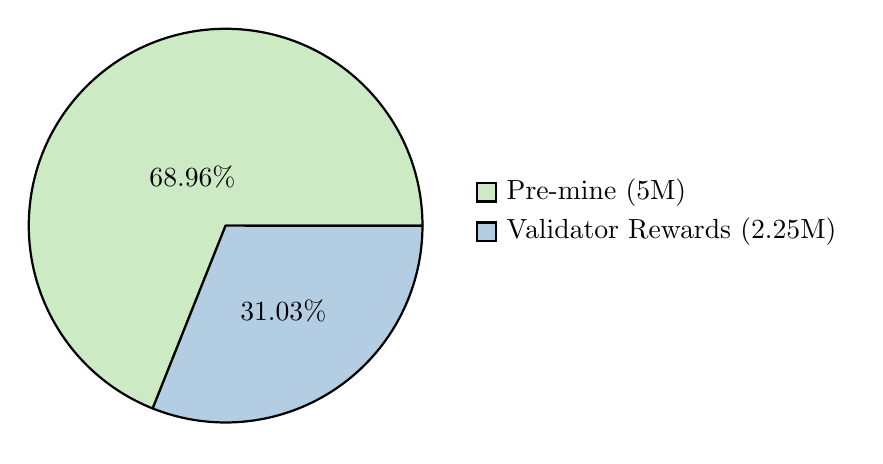
\begin{tikzpicture}
\pie[text = legend, align=center, radius=2.5, color = {
        category9,category10, }]{
68.96/Pre-mine (5M),
31.03/Validator Rewards (2.25M)
}
\end{tikzpicture}
\caption{Total Supply Distribution}
\end{figure}
\end{center}

\subsection{Inflation Model}

\begin{figure}[H]
\begin{center}
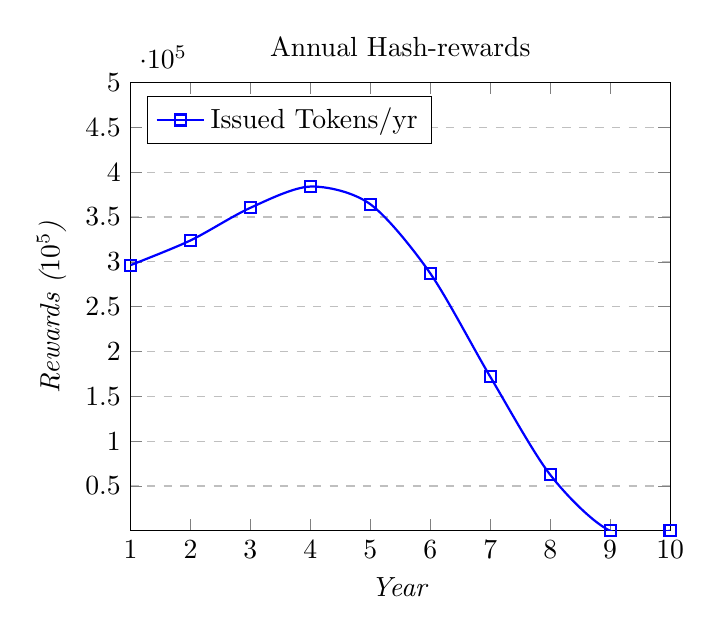
\begin{tikzpicture}
\begin{axis}[
    title={Annual Hash-rewards},
    xlabel={\textit{Year}},
    ylabel={\textit{Rewards ($10^5$)}},
    xmin=1, xmax=10,
    ymin=0, ymax=500000,
    xtick={1,2,3,4,5,6,7,8,9,10},
    ytick={50000,100000,150000,200000,250000,300000,350000,400000,450000,500000},
    legend pos=north west,
    ymajorgrids=true,
    grid style=dashed,
]

\addplot[
    color=blue,
    mark=square,smooth, thick
    ]
    coordinates {
    (1,296260.8337)(2,323825.8362)(3,360260.0098)(4,383911.1328)(5, 364257.8125)(6,287109.375)(7,171875)(8,62500)(9,0)(10,0)
    };
    \legend{Issued Tokens/yr}
    
\end{axis}
\end{tikzpicture}
\end{center}
\end{figure}

The Blinkcoin inflation model works on different method of supplying tokens "Hash-Rewards". This method can supply new coins according to the time spent by a block producer on validating and atteting the transactions to the block. The inflation is restricted to 9 years of time spent by validators on transactions- which may not be equal to standard time.

\begin{figure}[H]
\begin{center}
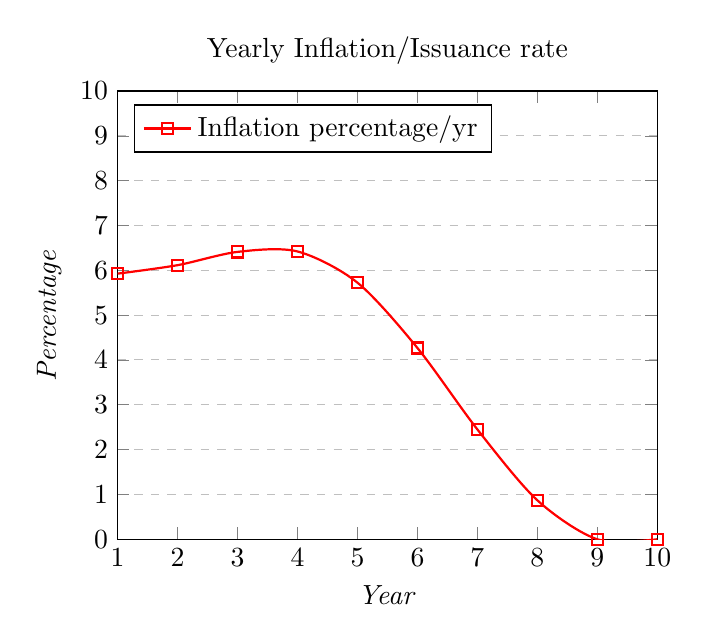
\begin{tikzpicture}
\begin{axis}[
    title={Yearly Inflation/Issuance rate},
    xlabel={\textit{Year}},
    ylabel={\textit{Percentage}},
    xmin=1, xmax=10,
    ymin=0, ymax=10,
    xtick={1,2,3,4,5,6,7,8,9,10},
    ytick={0,1,2,3,4,5,6,7,8,9,10},
    legend pos=north west,
    ymajorgrids=true,
    grid style=dashed,
]

\addplot[
    color=red,
    mark=square,smooth, thick
    ]
    coordinates {
    (1,5.925216675)(2,6.114235049)(3,6.410221602)(4,6.419546447)(5, 5.7234924045)(6,4.267053701)(7,2.449888641)(8,0.8695652174)(9,0)(10,0)
    };
    \legend{Inflation percentage/yr}
    
\end{axis}
\end{tikzpicture}
\end{center}
\end{figure}


The rewards are supplied in the network in an inverted Parabola curve from 5.93\% at the first year, where during the 4th and 5th the inflation is set to rise at peak of 6.42\% and falls linearly till 0 in the 9th year. The average issuance rate is set at 250,000 tokens per year, and the total inflation is 45\% for total 9 years supplying and saturating blinkcoins to many holders, delegators and validators essentially making the token much more decentralized in the long run.\\

\section{Token Sale}

\subsection{Private Sale}

- Close Sale
- Open Sale

\subsection{Public Sale}

\subsubsection{Initial Issue Price}

\subsubsection{Standard Currency}

\subsubsection{Currency Acceptance}

\subsubsection{Soft Cap}

\section{Token Allocation}

\begin{center}
\begin{figure}[H]
\centering
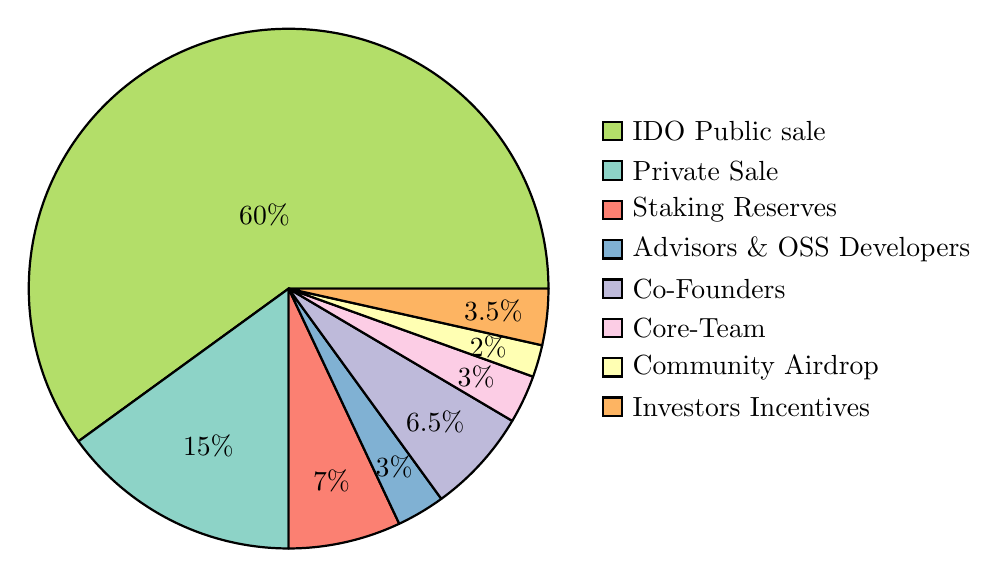
\begin{tikzpicture}
\pie[text = legend, align=center, radius = 3.3, color = {
        category7,category1,category4,category5,category3,
        category8, category2,category6,   },  
]{
60/IDO Public sale,
15/Private Sale,
7/Staking Reserves,
3/Advisors \& OSS Developers,
6.5/Co-Founders,
3/Core-Team,
2/Community Airdrop,
3.5/Investors Incentives
}
\end{tikzpicture}
\caption{Premined Token Distribution}
\end{figure}
\end{center}

\begin{table}[!ht]
    \centering
    \begin{tabular}{|c|c|}
    \hline
        \textbf{Description} & \textbf{Total Tokens} \\ \hline
        IDO Public Sale & 3,000,000\\
        Private Sale & 750,000\\
		Staking Reserves & 350,000 \\
		Advisors \& OSS Devs & 150,000 \\
		Co-Founders & 325,000 \\
		Core-Team & 150,000 \\
		Community & 100,000 \\
		Investors Incentive & 175,000 \\ \hline 
		\textbf{Total} & 5,000,000 \\ \hline \hline
		\textit{Vested Blinkcoins} & 900,000\\
        \textit{Non-Vested Blinkcoins} & 4,100,000\\ \hline
    \end{tabular}
\end{table}


\section{Vesting Period}

\begin{center}
\begin{figure}[H]\label{vest-nonvest}
\centering
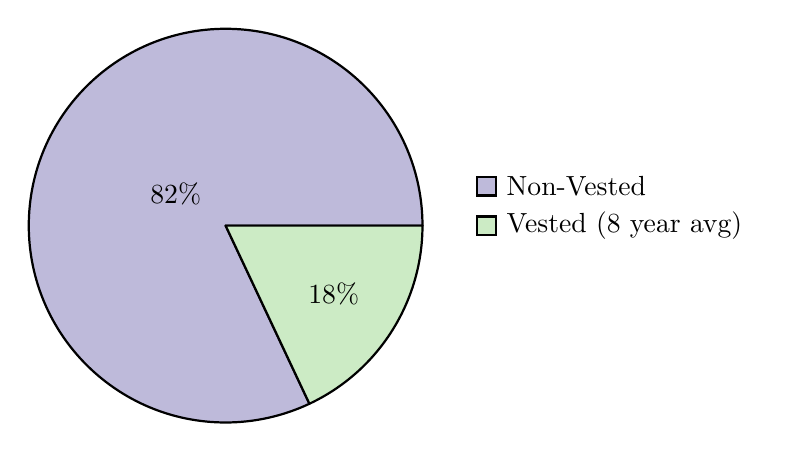
\begin{tikzpicture}
\pie[text = legend, align=center, radius = 2.5, color = {
        category3, category9,   },  
]{
82/Non-Vested,
18/ Vested (8 year avg)
}
\end{tikzpicture}
\caption{Vested-Non Vested}
\end{figure}
\end{center}

About 18\% of Premined 5 Million Blinkcoins will be subjected to a vesting period at an average of 8 years to avoid major-sell offs by the creators of the Project Blink and to receive positive-feedback from the public community. Figure 3 [\ref{vest-nonvest}] shows the difference in percentages of vested and non-vested blinkcoins.

\begin{center}
\begin{figure}[H]
\centering
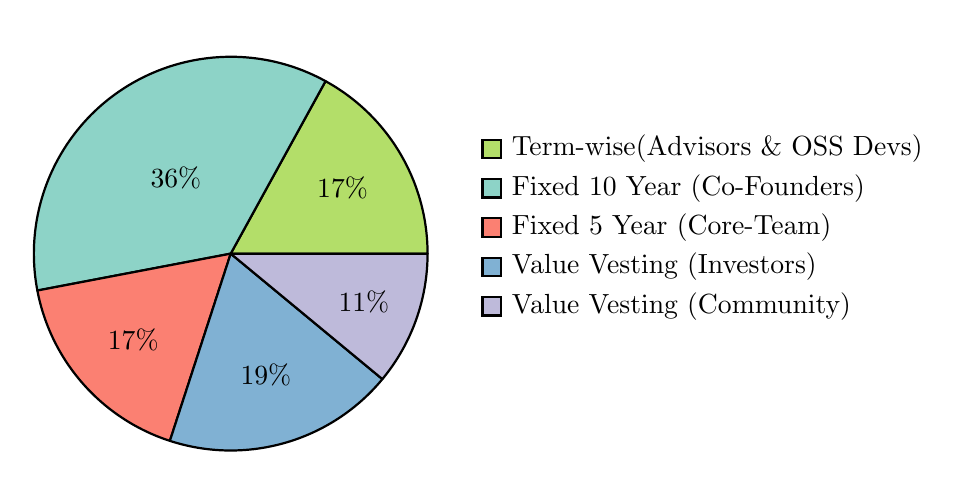
\begin{tikzpicture}
\pie[text = legend, align=center, radius = 2.5, color = {
       category7,category1,category4,category5,category3,
        category8, category2,category6, category11   },  
]{
17/Term-wise(Advisors \& OSS Devs),
36/Fixed 10 Year (Co-Founders),
17/Fixed 5 Year (Core-Team),
19/Value Vesting (Investors),
11/Value Vesting (Community)
}
\end{tikzpicture}
\caption{18\% Vesting Distribution}
\end{figure}
\end{center}

Vesting is classified into three categories initially,
\begin{enumerate}
\item \textbf{Fixed Vesting} - Tokens are vested normally for a fixed time period for fixed individuals with a withdrawal period e.g., 10k Tokens for 2 years with each month pay out
\item \textbf{Term-wise Vesting} - Similar to Fixed vesting but with flexible terms for different individuals
\item \textbf{Value Vesting} - Vesting payout based on blinkcoin's value appreciation e.g., 10k tokens where 5\% payout for 50\% increase in appreciation.
\end{enumerate}

Core-Team and Co-Founders of the project will undergo a fixed vesting schedule for a long period to gain confidence from the public and to voice about the long-term commitment for building a decentralized world bank. For Core-Team the vesting schedule is fixed at 5 years and Co-founders at 10 years.\\

Value Vesting is projected for Early Investors and Active Community members as an airdrop restricting major-sell offs on decentralized exchanges, for liquidity control. Investors here denoted are equity investors of the organization "Auguth Tech Pvt Ltd, India", who will avail incentive benefits for funding the development of Project Blink's Phase 1 - Blinkchain. Community members are selected with specific criteria of contribution in Social Handles such as Discord and are airdroped with the incentive tokens.\\

Term-wise vesting is a flexible schedule specifcally provided to short-term or goal-oriented individuals who can contribute on growing blinkchain into a regulated solution for world's finance and decentralized economy. Advisors and Open-Source Software developers are included in this vesting type and they can avail benefits of customized vesting oppurtunities.\\

\begin{enumerate}
\item \textit{Core-Team Contract}: 
\item \textit{Co-Founders Contract}: 
\item \textit{Advisors Contract}:
\end{enumerate}



\subsection{Non-Vested Distribution}

\begin{center}
\begin{figure}[H]
\centering
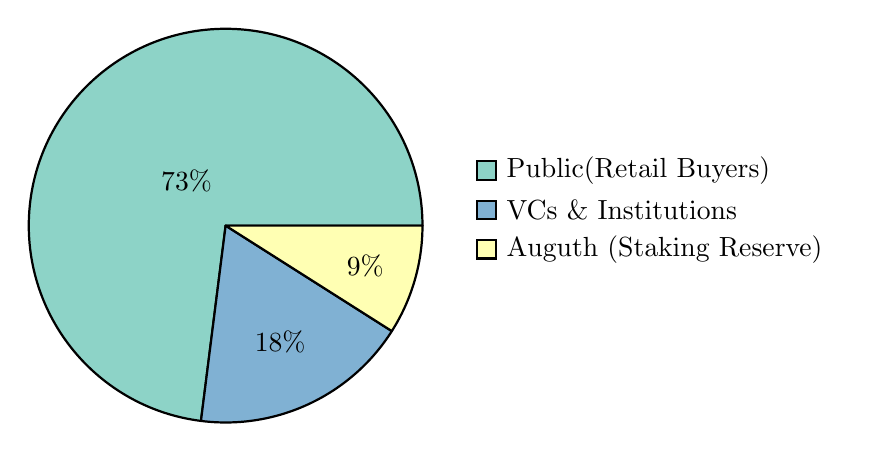
\begin{tikzpicture}
\pie[text = legend, align=center, radius = 2.5, color = {
       category1,category5, category2,   },  
]{
73/Public(Retail Buyers),
18/VCs \& Institutions,
9/Auguth (Staking Reserve)
}
\end{tikzpicture}
\caption{82\% Non-Vested Distribution}
\end{figure}
\end{center}

Non-vested distribution clearly will show the decentralized nature of blinkcoin, as its major 73\% will be sold to public. 18\% of the liquidity will be sold in Pre-sale to Ventures and Institutions. As the percentage of private holdings are negligible, and the allocations are fixed, the public holders can avail benefits of pure decentralization. 9\% of the liquid tokens will be hold for staking reserves for bootstrapping the native chain. The reserves are kept for purely staking demand, and shall not be used as a compensation for any team members or co-founders. The income from staking rewards and its expenditures are decided by the centralized entity which holds the reserves.

\section{Use of Sale Proceeds}

\subsection{Capital Collected}

\subsection{Technical}

\subsection{Non-Technical}




\end{document}